%%%%%%%%%%%%%%%%%%%%%%%%%%%%%%%%%%%%%%%%%
% Tecnológico de Costa Rica/Instructivo de Laboratorio de Instrumentación I
% LaTeX Template
% Version 3.1 (25/3/14)
%
% This template has been downloaded from:
% http://www.LaTeXTemplates.com
%
% Original author:
% Linux and Unix Users Group at Virginia Tech Wiki 
% (https://vtluug.org/wiki/Example_LaTeX_chem_lab_report)
%
% License:
% CC BY-NC-SA 3.0 (http://creativecommons.org/licenses/by-nc-sa/3.0/)
%
%%%%%%%%%%%%%%%%%%%%%%%%%%%%%%%%%%%%%%%%%

%----------------------------------------------------------------------------------------
%	PACKAGES AND DOCUMENT CONFIGURATIONS
%----------------------------------------------------------------------------------------

\documentclass[12pt,letterpaper]{report}
\usepackage{amsmath}
\usepackage{amssymb}
\usepackage{siunitx}
\usepackage{float}
\usepackage{tikz}
\def\checkmark{\tikz\fill[scale=0.4](0,.35) -- (.25,0) -- (1,.7) -- (.25,.15) -- cycle;} 
\usepackage{url}
\usepackage[siunitx,american,RPvoltages]{circuitikz}
\ctikzset{capacitors/scale=0.7}
\ctikzset{diodes/scale=0.7}
\usepackage{tabularx}
\newcolumntype{C}{>{\centering\arraybackslash}X}
\renewcommand\tabularxcolumn[1]{m{#1}}% for vertical centering text in X column
\usepackage{tabu}
\usepackage[spanish,es-tabla,activeacute]{babel}
\usepackage{babelbib}
\usepackage{booktabs}
\usepackage{pgfplots}
\usepackage{hyperref}
\hypersetup{colorlinks = true,
            linkcolor = black,
            urlcolor  = blue,
            citecolor = blue,
            anchorcolor = blue}
\usepgfplotslibrary{units, fillbetween} 
\pgfplotsset{compat=1.16}
\usepackage{bm}
\usetikzlibrary{arrows, arrows.meta, shapes, 3d, perspective, positioning,mindmap,trees,backgrounds}
\renewcommand{\sin}{\sen} %change from sin to sen
\usepackage{bohr}
\setbohr{distribution-method = quantum,insert-missing = true}
\usepackage{elements}
\usepackage{verbatim}
\usepackage[edges]{forest}
\usepackage{etoolbox}
\usepackage{schemata}
\usepackage{appendix}
\usepackage{listings}

\definecolor{color_mate}{RGB}{255,255,128}
\definecolor{color_plas}{RGB}{255,128,255}
\definecolor{color_text}{RGB}{128,255,255}
\definecolor{color_petr}{RGB}{255,192,192}
\definecolor{color_made}{RGB}{192,255,192}
\definecolor{color_meta}{RGB}{192,192,255}
\newcommand\diagram[2]{\schema{\schemabox{#1}}{\schemabox{#2}}}

\definecolor{codegreen}{rgb}{0,0.6,0}
\definecolor{codegray}{rgb}{0.5,0.5,0.5}
\definecolor{codepurple}{rgb}{0.58,0,0.82}
\definecolor{backcolour}{rgb}{0.95,0.95,0.92}

\lstdefinestyle{mystyle}{
    backgroundcolor=\color{backcolour},   
    commentstyle=\color{codegreen},
    keywordstyle=\color{magenta},
    numberstyle=\tiny\color{codegray},
    stringstyle=\color{codepurple},
    basicstyle=\ttfamily\footnotesize,
    breakatwhitespace=false,         
    breaklines=true,                 
    captionpos=b,                    
    keepspaces=true,                 
    numbers=left,                    
    numbersep=5pt,                  
    showspaces=false,                
    showstringspaces=false,
    showtabs=false,                  
    tabsize=2
}

\lstset{style=mystyle}
%%%%%%%%%%%%%%%%%%%%%%%%%%%%%%%%%%%%%%%%%%%%%%%%%%%%%%%%%%%%%%%%%%%%%%%%%%%%%%%% 
%%% ~ Arduino Language - Arduino IDE Colors ~                                  %%%
%%%                                                                            %%%
%%% Kyle Rocha-Brownell | 10/2/2017 | No Licence                               %%%
%%% -------------------------------------------------------------------------- %%%
%%%                                                                            %%%
%%% Place this file in your working directory (next to the latex file you're   %%%
%%% working on).  To add it to your project, place:                            %%%
%%%    %%%%%%%%%%%%%%%%%%%%%%%%%%%%%%%%%%%%%%%%%%%%%%%%%%%%%%%%%%%%%%%%%%%%%%%%%%%%%%%% 
%%% ~ Arduino Language - Arduino IDE Colors ~                                  %%%
%%%                                                                            %%%
%%% Kyle Rocha-Brownell | 10/2/2017 | No Licence                               %%%
%%% -------------------------------------------------------------------------- %%%
%%%                                                                            %%%
%%% Place this file in your working directory (next to the latex file you're   %%%
%%% working on).  To add it to your project, place:                            %%%
%%%    %%%%%%%%%%%%%%%%%%%%%%%%%%%%%%%%%%%%%%%%%%%%%%%%%%%%%%%%%%%%%%%%%%%%%%%%%%%%%%%% 
%%% ~ Arduino Language - Arduino IDE Colors ~                                  %%%
%%%                                                                            %%%
%%% Kyle Rocha-Brownell | 10/2/2017 | No Licence                               %%%
%%% -------------------------------------------------------------------------- %%%
%%%                                                                            %%%
%%% Place this file in your working directory (next to the latex file you're   %%%
%%% working on).  To add it to your project, place:                            %%%
%%%    \input{arduinoLanguage.tex}                                             %%%
%%% somewhere before \begin{document} in your latex file.                      %%%
%%%                                                                            %%%
%%% In your document, place your arduino code between:                         %%%
%%%   \begin{lstlisting}[language=Arduino]                                     %%%
%%% and:                                                                       %%%
%%%   \end{lstlisting}                                                         %%%
%%%                                                                            %%%
%%% Or create your own style to add non-built-in functions and variables.      %%%
%%%                                                                            %%%
 %%%%%%%%%%%%%%%%%%%%%%%%%%%%%%%%%%%%%%%%%%%%%%%%%%%%%%%%%%%%%%%%%%%%%%%%%%%%%%%% 

\usepackage{color}
\usepackage{listings}    
\usepackage{courier}

%%% Define Custom IDE Colors %%%
\definecolor{arduinoGreen}    {rgb} {0.17, 0.43, 0.01}
\definecolor{arduinoGrey}     {rgb} {0.47, 0.47, 0.33}
\definecolor{arduinoOrange}   {rgb} {0.8 , 0.4 , 0   }
\definecolor{arduinoBlue}     {rgb} {0.01, 0.61, 0.98}
\definecolor{arduinoDarkBlue} {rgb} {0.0 , 0.2 , 0.5 }

%%% Define Arduino Language %%%
\lstdefinelanguage{Arduino}{
  language=C++, % begin with default C++ settings 
%
%
  %%% Keyword Color Group 1 %%%  (called KEYWORD3 by arduino)
  keywordstyle=\color{arduinoGreen},   
  deletekeywords={  % remove all arduino keywords that might be in c++
                break, case, override, final, continue, default, do, else, for, 
                if, return, goto, switch, throw, try, while, setup, loop, export, 
                not, or, and, xor, include, define, elif, else, error, if, ifdef, 
                ifndef, pragma, warning,
                HIGH, LOW, INPUT, INPUT_PULLUP, OUTPUT, DEC, BIN, HEX, OCT, PI, 
                HALF_PI, TWO_PI, LSBFIRST, MSBFIRST, CHANGE, FALLING, RISING, 
                DEFAULT, EXTERNAL, INTERNAL, INTERNAL1V1, INTERNAL2V56, LED_BUILTIN, 
                LED_BUILTIN_RX, LED_BUILTIN_TX, DIGITAL_MESSAGE, FIRMATA_STRING, 
                ANALOG_MESSAGE, REPORT_DIGITAL, REPORT_ANALOG, SET_PIN_MODE, 
                SYSTEM_RESET, SYSEX_START, auto, int8_t, int16_t, int32_t, int64_t, 
                uint8_t, uint16_t, uint32_t, uint64_t, char16_t, char32_t, operator, 
                enum, delete, bool, boolean, byte, char, const, false, float, double, 
                null, NULL, int, long, new, private, protected, public, short, 
                signed, static, volatile, String, void, true, unsigned, word, array, 
                sizeof, dynamic_cast, typedef, const_cast, struct, static_cast, union, 
                friend, extern, class, reinterpret_cast, register, explicit, inline, 
                _Bool, complex, _Complex, _Imaginary, atomic_bool, atomic_char, 
                atomic_schar, atomic_uchar, atomic_short, atomic_ushort, atomic_int, 
                atomic_uint, atomic_long, atomic_ulong, atomic_llong, atomic_ullong, 
                virtual, PROGMEM,
                Serial, Serial1, Serial2, Serial3, SerialUSB, Keyboard, Mouse,
                abs, acos, asin, atan, atan2, ceil, constrain, cos, degrees, exp, 
                floor, log, map, max, min, radians, random, randomSeed, round, sin, 
                sq, sqrt, tan, pow, bitRead, bitWrite, bitSet, bitClear, bit, 
                highByte, lowByte, analogReference, analogRead, 
                analogReadResolution, analogWrite, analogWriteResolution, 
                attachInterrupt, detachInterrupt, digitalPinToInterrupt, delay, 
                delayMicroseconds, digitalWrite, digitalRead, interrupts, millis, 
                micros, noInterrupts, noTone, pinMode, pulseIn, pulseInLong, shiftIn, 
                shiftOut, tone, yield, Stream, begin, end, peek, read, print, 
                println, available, availableForWrite, flush, setTimeout, find, 
                findUntil, parseInt, parseFloat, readBytes, readBytesUntil, readString, 
                readStringUntil, trim, toUpperCase, toLowerCase, charAt, compareTo, 
                concat, endsWith, startsWith, equals, equalsIgnoreCase, getBytes, 
                indexOf, lastIndexOf, length, replace, setCharAt, substring, 
                toCharArray, toInt, press, release, releaseAll, accept, click, move, 
                isPressed, isAlphaNumeric, isAlpha, isAscii, isWhitespace, isControl, 
                isDigit, isGraph, isLowerCase, isPrintable, isPunct, isSpace, 
                isUpperCase, isHexadecimalDigit, 
                }, 
  morekeywords={   % add arduino structures to group 1
                break, case, override, final, continue, default, do, else, for, 
                if, return, goto, switch, throw, try, while, setup, loop, export, 
                not, or, and, xor, include, define, elif, else, error, if, ifdef, 
                ifndef, pragma, warning,
                }, 
% 
%
  %%% Keyword Color Group 2 %%%  (called LITERAL1 by arduino)
  keywordstyle=[2]\color{arduinoBlue},   
  keywords=[2]{   % add variables and dataTypes as 2nd group  
                HIGH, LOW, INPUT, INPUT_PULLUP, OUTPUT, DEC, BIN, HEX, OCT, PI, 
                HALF_PI, TWO_PI, LSBFIRST, MSBFIRST, CHANGE, FALLING, RISING, 
                DEFAULT, EXTERNAL, INTERNAL, INTERNAL1V1, INTERNAL2V56, LED_BUILTIN, 
                LED_BUILTIN_RX, LED_BUILTIN_TX, DIGITAL_MESSAGE, FIRMATA_STRING, 
                ANALOG_MESSAGE, REPORT_DIGITAL, REPORT_ANALOG, SET_PIN_MODE, 
                SYSTEM_RESET, SYSEX_START, auto, int8_t, int16_t, int32_t, int64_t, 
                uint8_t, uint16_t, uint32_t, uint64_t, char16_t, char32_t, operator, 
                enum, delete, bool, boolean, byte, char, const, false, float, double, 
                null, NULL, int, long, new, private, protected, public, short, 
                signed, static, volatile, String, void, true, unsigned, word, array, 
                sizeof, dynamic_cast, typedef, const_cast, struct, static_cast, union, 
                friend, extern, class, reinterpret_cast, register, explicit, inline, 
                _Bool, complex, _Complex, _Imaginary, atomic_bool, atomic_char, 
                atomic_schar, atomic_uchar, atomic_short, atomic_ushort, atomic_int, 
                atomic_uint, atomic_long, atomic_ulong, atomic_llong, atomic_ullong, 
                virtual, PROGMEM,
                },  
% 
%
  %%% Keyword Color Group 3 %%%  (called KEYWORD1 by arduino)
  keywordstyle=[3]\bfseries\color{arduinoOrange},
  keywords=[3]{  % add built-in functions as a 3rd group
                Serial, Serial1, Serial2, Serial3, SerialUSB, Keyboard, Mouse,
                },      
%
%
  %%% Keyword Color Group 4 %%%  (called KEYWORD2 by arduino)
  keywordstyle=[4]\color{arduinoOrange},
  keywords=[4]{  % add more built-in functions as a 4th group
                abs, acos, asin, atan, atan2, ceil, constrain, cos, degrees, exp, 
                floor, log, map, max, min, radians, random, randomSeed, round, sin, 
                sq, sqrt, tan, pow, bitRead, bitWrite, bitSet, bitClear, bit, 
                highByte, lowByte, analogReference, analogRead, 
                analogReadResolution, analogWrite, analogWriteResolution, 
                attachInterrupt, detachInterrupt, digitalPinToInterrupt, delay, 
                delayMicroseconds, digitalWrite, digitalRead, interrupts, millis, 
                micros, noInterrupts, noTone, pinMode, pulseIn, pulseInLong, shiftIn, 
                shiftOut, tone, yield, Stream, begin, end, peek, read, print, 
                println, available, availableForWrite, flush, setTimeout, find, 
                findUntil, parseInt, parseFloat, readBytes, readBytesUntil, readString, 
                readStringUntil, trim, toUpperCase, toLowerCase, charAt, compareTo, 
                concat, endsWith, startsWith, equals, equalsIgnoreCase, getBytes, 
                indexOf, lastIndexOf, length, replace, setCharAt, substring, 
                toCharArray, toInt, press, release, releaseAll, accept, click, move, 
                isPressed, isAlphaNumeric, isAlpha, isAscii, isWhitespace, isControl, 
                isDigit, isGraph, isLowerCase, isPrintable, isPunct, isSpace, 
                isUpperCase, isHexadecimalDigit, 
                },      
%
%
  %%% Set Other Colors %%%
  stringstyle=\color{arduinoDarkBlue},    
  commentstyle=\color{arduinoGrey},    
%          
%   
  %%%% Line Numbering %%%%
   numbers=left,                    
  numbersep=5pt,                   
  numberstyle=\color{arduinoGrey},    
  %stepnumber=2,                      % show every 2 line numbers
%
%
  %%%% Code Box Style %%%%
  breaklines=true,                    % wordwrapping
  tabsize=2,         
  basicstyle=\ttfamily\footnotesize
}                                             %%%
%%% somewhere before \begin{document} in your latex file.                      %%%
%%%                                                                            %%%
%%% In your document, place your arduino code between:                         %%%
%%%   \begin{lstlisting}[language=Arduino]                                     %%%
%%% and:                                                                       %%%
%%%   \end{lstlisting}                                                         %%%
%%%                                                                            %%%
%%% Or create your own style to add non-built-in functions and variables.      %%%
%%%                                                                            %%%
 %%%%%%%%%%%%%%%%%%%%%%%%%%%%%%%%%%%%%%%%%%%%%%%%%%%%%%%%%%%%%%%%%%%%%%%%%%%%%%%% 

\usepackage{color}
\usepackage{listings}    
\usepackage{courier}

%%% Define Custom IDE Colors %%%
\definecolor{arduinoGreen}    {rgb} {0.17, 0.43, 0.01}
\definecolor{arduinoGrey}     {rgb} {0.47, 0.47, 0.33}
\definecolor{arduinoOrange}   {rgb} {0.8 , 0.4 , 0   }
\definecolor{arduinoBlue}     {rgb} {0.01, 0.61, 0.98}
\definecolor{arduinoDarkBlue} {rgb} {0.0 , 0.2 , 0.5 }

%%% Define Arduino Language %%%
\lstdefinelanguage{Arduino}{
  language=C++, % begin with default C++ settings 
%
%
  %%% Keyword Color Group 1 %%%  (called KEYWORD3 by arduino)
  keywordstyle=\color{arduinoGreen},   
  deletekeywords={  % remove all arduino keywords that might be in c++
                break, case, override, final, continue, default, do, else, for, 
                if, return, goto, switch, throw, try, while, setup, loop, export, 
                not, or, and, xor, include, define, elif, else, error, if, ifdef, 
                ifndef, pragma, warning,
                HIGH, LOW, INPUT, INPUT_PULLUP, OUTPUT, DEC, BIN, HEX, OCT, PI, 
                HALF_PI, TWO_PI, LSBFIRST, MSBFIRST, CHANGE, FALLING, RISING, 
                DEFAULT, EXTERNAL, INTERNAL, INTERNAL1V1, INTERNAL2V56, LED_BUILTIN, 
                LED_BUILTIN_RX, LED_BUILTIN_TX, DIGITAL_MESSAGE, FIRMATA_STRING, 
                ANALOG_MESSAGE, REPORT_DIGITAL, REPORT_ANALOG, SET_PIN_MODE, 
                SYSTEM_RESET, SYSEX_START, auto, int8_t, int16_t, int32_t, int64_t, 
                uint8_t, uint16_t, uint32_t, uint64_t, char16_t, char32_t, operator, 
                enum, delete, bool, boolean, byte, char, const, false, float, double, 
                null, NULL, int, long, new, private, protected, public, short, 
                signed, static, volatile, String, void, true, unsigned, word, array, 
                sizeof, dynamic_cast, typedef, const_cast, struct, static_cast, union, 
                friend, extern, class, reinterpret_cast, register, explicit, inline, 
                _Bool, complex, _Complex, _Imaginary, atomic_bool, atomic_char, 
                atomic_schar, atomic_uchar, atomic_short, atomic_ushort, atomic_int, 
                atomic_uint, atomic_long, atomic_ulong, atomic_llong, atomic_ullong, 
                virtual, PROGMEM,
                Serial, Serial1, Serial2, Serial3, SerialUSB, Keyboard, Mouse,
                abs, acos, asin, atan, atan2, ceil, constrain, cos, degrees, exp, 
                floor, log, map, max, min, radians, random, randomSeed, round, sin, 
                sq, sqrt, tan, pow, bitRead, bitWrite, bitSet, bitClear, bit, 
                highByte, lowByte, analogReference, analogRead, 
                analogReadResolution, analogWrite, analogWriteResolution, 
                attachInterrupt, detachInterrupt, digitalPinToInterrupt, delay, 
                delayMicroseconds, digitalWrite, digitalRead, interrupts, millis, 
                micros, noInterrupts, noTone, pinMode, pulseIn, pulseInLong, shiftIn, 
                shiftOut, tone, yield, Stream, begin, end, peek, read, print, 
                println, available, availableForWrite, flush, setTimeout, find, 
                findUntil, parseInt, parseFloat, readBytes, readBytesUntil, readString, 
                readStringUntil, trim, toUpperCase, toLowerCase, charAt, compareTo, 
                concat, endsWith, startsWith, equals, equalsIgnoreCase, getBytes, 
                indexOf, lastIndexOf, length, replace, setCharAt, substring, 
                toCharArray, toInt, press, release, releaseAll, accept, click, move, 
                isPressed, isAlphaNumeric, isAlpha, isAscii, isWhitespace, isControl, 
                isDigit, isGraph, isLowerCase, isPrintable, isPunct, isSpace, 
                isUpperCase, isHexadecimalDigit, 
                }, 
  morekeywords={   % add arduino structures to group 1
                break, case, override, final, continue, default, do, else, for, 
                if, return, goto, switch, throw, try, while, setup, loop, export, 
                not, or, and, xor, include, define, elif, else, error, if, ifdef, 
                ifndef, pragma, warning,
                }, 
% 
%
  %%% Keyword Color Group 2 %%%  (called LITERAL1 by arduino)
  keywordstyle=[2]\color{arduinoBlue},   
  keywords=[2]{   % add variables and dataTypes as 2nd group  
                HIGH, LOW, INPUT, INPUT_PULLUP, OUTPUT, DEC, BIN, HEX, OCT, PI, 
                HALF_PI, TWO_PI, LSBFIRST, MSBFIRST, CHANGE, FALLING, RISING, 
                DEFAULT, EXTERNAL, INTERNAL, INTERNAL1V1, INTERNAL2V56, LED_BUILTIN, 
                LED_BUILTIN_RX, LED_BUILTIN_TX, DIGITAL_MESSAGE, FIRMATA_STRING, 
                ANALOG_MESSAGE, REPORT_DIGITAL, REPORT_ANALOG, SET_PIN_MODE, 
                SYSTEM_RESET, SYSEX_START, auto, int8_t, int16_t, int32_t, int64_t, 
                uint8_t, uint16_t, uint32_t, uint64_t, char16_t, char32_t, operator, 
                enum, delete, bool, boolean, byte, char, const, false, float, double, 
                null, NULL, int, long, new, private, protected, public, short, 
                signed, static, volatile, String, void, true, unsigned, word, array, 
                sizeof, dynamic_cast, typedef, const_cast, struct, static_cast, union, 
                friend, extern, class, reinterpret_cast, register, explicit, inline, 
                _Bool, complex, _Complex, _Imaginary, atomic_bool, atomic_char, 
                atomic_schar, atomic_uchar, atomic_short, atomic_ushort, atomic_int, 
                atomic_uint, atomic_long, atomic_ulong, atomic_llong, atomic_ullong, 
                virtual, PROGMEM,
                },  
% 
%
  %%% Keyword Color Group 3 %%%  (called KEYWORD1 by arduino)
  keywordstyle=[3]\bfseries\color{arduinoOrange},
  keywords=[3]{  % add built-in functions as a 3rd group
                Serial, Serial1, Serial2, Serial3, SerialUSB, Keyboard, Mouse,
                },      
%
%
  %%% Keyword Color Group 4 %%%  (called KEYWORD2 by arduino)
  keywordstyle=[4]\color{arduinoOrange},
  keywords=[4]{  % add more built-in functions as a 4th group
                abs, acos, asin, atan, atan2, ceil, constrain, cos, degrees, exp, 
                floor, log, map, max, min, radians, random, randomSeed, round, sin, 
                sq, sqrt, tan, pow, bitRead, bitWrite, bitSet, bitClear, bit, 
                highByte, lowByte, analogReference, analogRead, 
                analogReadResolution, analogWrite, analogWriteResolution, 
                attachInterrupt, detachInterrupt, digitalPinToInterrupt, delay, 
                delayMicroseconds, digitalWrite, digitalRead, interrupts, millis, 
                micros, noInterrupts, noTone, pinMode, pulseIn, pulseInLong, shiftIn, 
                shiftOut, tone, yield, Stream, begin, end, peek, read, print, 
                println, available, availableForWrite, flush, setTimeout, find, 
                findUntil, parseInt, parseFloat, readBytes, readBytesUntil, readString, 
                readStringUntil, trim, toUpperCase, toLowerCase, charAt, compareTo, 
                concat, endsWith, startsWith, equals, equalsIgnoreCase, getBytes, 
                indexOf, lastIndexOf, length, replace, setCharAt, substring, 
                toCharArray, toInt, press, release, releaseAll, accept, click, move, 
                isPressed, isAlphaNumeric, isAlpha, isAscii, isWhitespace, isControl, 
                isDigit, isGraph, isLowerCase, isPrintable, isPunct, isSpace, 
                isUpperCase, isHexadecimalDigit, 
                },      
%
%
  %%% Set Other Colors %%%
  stringstyle=\color{arduinoDarkBlue},    
  commentstyle=\color{arduinoGrey},    
%          
%   
  %%%% Line Numbering %%%%
   numbers=left,                    
  numbersep=5pt,                   
  numberstyle=\color{arduinoGrey},    
  %stepnumber=2,                      % show every 2 line numbers
%
%
  %%%% Code Box Style %%%%
  breaklines=true,                    % wordwrapping
  tabsize=2,         
  basicstyle=\ttfamily\footnotesize
}                                             %%%
%%% somewhere before \begin{document} in your latex file.                      %%%
%%%                                                                            %%%
%%% In your document, place your arduino code between:                         %%%
%%%   \begin{lstlisting}[language=Arduino]                                     %%%
%%% and:                                                                       %%%
%%%   \end{lstlisting}                                                         %%%
%%%                                                                            %%%
%%% Or create your own style to add non-built-in functions and variables.      %%%
%%%                                                                            %%%
 %%%%%%%%%%%%%%%%%%%%%%%%%%%%%%%%%%%%%%%%%%%%%%%%%%%%%%%%%%%%%%%%%%%%%%%%%%%%%%%% 

\usepackage{color}
\usepackage{listings}    
\usepackage{courier}

%%% Define Custom IDE Colors %%%
\definecolor{arduinoGreen}    {rgb} {0.17, 0.43, 0.01}
\definecolor{arduinoGrey}     {rgb} {0.47, 0.47, 0.33}
\definecolor{arduinoOrange}   {rgb} {0.8 , 0.4 , 0   }
\definecolor{arduinoBlue}     {rgb} {0.01, 0.61, 0.98}
\definecolor{arduinoDarkBlue} {rgb} {0.0 , 0.2 , 0.5 }

%%% Define Arduino Language %%%
\lstdefinelanguage{Arduino}{
  language=C++, % begin with default C++ settings 
%
%
  %%% Keyword Color Group 1 %%%  (called KEYWORD3 by arduino)
  keywordstyle=\color{arduinoGreen},   
  deletekeywords={  % remove all arduino keywords that might be in c++
                break, case, override, final, continue, default, do, else, for, 
                if, return, goto, switch, throw, try, while, setup, loop, export, 
                not, or, and, xor, include, define, elif, else, error, if, ifdef, 
                ifndef, pragma, warning,
                HIGH, LOW, INPUT, INPUT_PULLUP, OUTPUT, DEC, BIN, HEX, OCT, PI, 
                HALF_PI, TWO_PI, LSBFIRST, MSBFIRST, CHANGE, FALLING, RISING, 
                DEFAULT, EXTERNAL, INTERNAL, INTERNAL1V1, INTERNAL2V56, LED_BUILTIN, 
                LED_BUILTIN_RX, LED_BUILTIN_TX, DIGITAL_MESSAGE, FIRMATA_STRING, 
                ANALOG_MESSAGE, REPORT_DIGITAL, REPORT_ANALOG, SET_PIN_MODE, 
                SYSTEM_RESET, SYSEX_START, auto, int8_t, int16_t, int32_t, int64_t, 
                uint8_t, uint16_t, uint32_t, uint64_t, char16_t, char32_t, operator, 
                enum, delete, bool, boolean, byte, char, const, false, float, double, 
                null, NULL, int, long, new, private, protected, public, short, 
                signed, static, volatile, String, void, true, unsigned, word, array, 
                sizeof, dynamic_cast, typedef, const_cast, struct, static_cast, union, 
                friend, extern, class, reinterpret_cast, register, explicit, inline, 
                _Bool, complex, _Complex, _Imaginary, atomic_bool, atomic_char, 
                atomic_schar, atomic_uchar, atomic_short, atomic_ushort, atomic_int, 
                atomic_uint, atomic_long, atomic_ulong, atomic_llong, atomic_ullong, 
                virtual, PROGMEM,
                Serial, Serial1, Serial2, Serial3, SerialUSB, Keyboard, Mouse,
                abs, acos, asin, atan, atan2, ceil, constrain, cos, degrees, exp, 
                floor, log, map, max, min, radians, random, randomSeed, round, sin, 
                sq, sqrt, tan, pow, bitRead, bitWrite, bitSet, bitClear, bit, 
                highByte, lowByte, analogReference, analogRead, 
                analogReadResolution, analogWrite, analogWriteResolution, 
                attachInterrupt, detachInterrupt, digitalPinToInterrupt, delay, 
                delayMicroseconds, digitalWrite, digitalRead, interrupts, millis, 
                micros, noInterrupts, noTone, pinMode, pulseIn, pulseInLong, shiftIn, 
                shiftOut, tone, yield, Stream, begin, end, peek, read, print, 
                println, available, availableForWrite, flush, setTimeout, find, 
                findUntil, parseInt, parseFloat, readBytes, readBytesUntil, readString, 
                readStringUntil, trim, toUpperCase, toLowerCase, charAt, compareTo, 
                concat, endsWith, startsWith, equals, equalsIgnoreCase, getBytes, 
                indexOf, lastIndexOf, length, replace, setCharAt, substring, 
                toCharArray, toInt, press, release, releaseAll, accept, click, move, 
                isPressed, isAlphaNumeric, isAlpha, isAscii, isWhitespace, isControl, 
                isDigit, isGraph, isLowerCase, isPrintable, isPunct, isSpace, 
                isUpperCase, isHexadecimalDigit, 
                }, 
  morekeywords={   % add arduino structures to group 1
                break, case, override, final, continue, default, do, else, for, 
                if, return, goto, switch, throw, try, while, setup, loop, export, 
                not, or, and, xor, include, define, elif, else, error, if, ifdef, 
                ifndef, pragma, warning,
                }, 
% 
%
  %%% Keyword Color Group 2 %%%  (called LITERAL1 by arduino)
  keywordstyle=[2]\color{arduinoBlue},   
  keywords=[2]{   % add variables and dataTypes as 2nd group  
                HIGH, LOW, INPUT, INPUT_PULLUP, OUTPUT, DEC, BIN, HEX, OCT, PI, 
                HALF_PI, TWO_PI, LSBFIRST, MSBFIRST, CHANGE, FALLING, RISING, 
                DEFAULT, EXTERNAL, INTERNAL, INTERNAL1V1, INTERNAL2V56, LED_BUILTIN, 
                LED_BUILTIN_RX, LED_BUILTIN_TX, DIGITAL_MESSAGE, FIRMATA_STRING, 
                ANALOG_MESSAGE, REPORT_DIGITAL, REPORT_ANALOG, SET_PIN_MODE, 
                SYSTEM_RESET, SYSEX_START, auto, int8_t, int16_t, int32_t, int64_t, 
                uint8_t, uint16_t, uint32_t, uint64_t, char16_t, char32_t, operator, 
                enum, delete, bool, boolean, byte, char, const, false, float, double, 
                null, NULL, int, long, new, private, protected, public, short, 
                signed, static, volatile, String, void, true, unsigned, word, array, 
                sizeof, dynamic_cast, typedef, const_cast, struct, static_cast, union, 
                friend, extern, class, reinterpret_cast, register, explicit, inline, 
                _Bool, complex, _Complex, _Imaginary, atomic_bool, atomic_char, 
                atomic_schar, atomic_uchar, atomic_short, atomic_ushort, atomic_int, 
                atomic_uint, atomic_long, atomic_ulong, atomic_llong, atomic_ullong, 
                virtual, PROGMEM,
                },  
% 
%
  %%% Keyword Color Group 3 %%%  (called KEYWORD1 by arduino)
  keywordstyle=[3]\bfseries\color{arduinoOrange},
  keywords=[3]{  % add built-in functions as a 3rd group
                Serial, Serial1, Serial2, Serial3, SerialUSB, Keyboard, Mouse,
                },      
%
%
  %%% Keyword Color Group 4 %%%  (called KEYWORD2 by arduino)
  keywordstyle=[4]\color{arduinoOrange},
  keywords=[4]{  % add more built-in functions as a 4th group
                abs, acos, asin, atan, atan2, ceil, constrain, cos, degrees, exp, 
                floor, log, map, max, min, radians, random, randomSeed, round, sin, 
                sq, sqrt, tan, pow, bitRead, bitWrite, bitSet, bitClear, bit, 
                highByte, lowByte, analogReference, analogRead, 
                analogReadResolution, analogWrite, analogWriteResolution, 
                attachInterrupt, detachInterrupt, digitalPinToInterrupt, delay, 
                delayMicroseconds, digitalWrite, digitalRead, interrupts, millis, 
                micros, noInterrupts, noTone, pinMode, pulseIn, pulseInLong, shiftIn, 
                shiftOut, tone, yield, Stream, begin, end, peek, read, print, 
                println, available, availableForWrite, flush, setTimeout, find, 
                findUntil, parseInt, parseFloat, readBytes, readBytesUntil, readString, 
                readStringUntil, trim, toUpperCase, toLowerCase, charAt, compareTo, 
                concat, endsWith, startsWith, equals, equalsIgnoreCase, getBytes, 
                indexOf, lastIndexOf, length, replace, setCharAt, substring, 
                toCharArray, toInt, press, release, releaseAll, accept, click, move, 
                isPressed, isAlphaNumeric, isAlpha, isAscii, isWhitespace, isControl, 
                isDigit, isGraph, isLowerCase, isPrintable, isPunct, isSpace, 
                isUpperCase, isHexadecimalDigit, 
                },      
%
%
  %%% Set Other Colors %%%
  stringstyle=\color{arduinoDarkBlue},    
  commentstyle=\color{arduinoGrey},    
%          
%   
  %%%% Line Numbering %%%%
   numbers=left,                    
  numbersep=5pt,                   
  numberstyle=\color{arduinoGrey},    
  %stepnumber=2,                      % show every 2 line numbers
%
%
  %%%% Code Box Style %%%%
  breaklines=true,                    % wordwrapping
  tabsize=2,         
  basicstyle=\ttfamily\footnotesize
}
\usepackage{csvsimple}
\usepackage{geometry} 
\geometry{left=18mm,right=18mm,top=21mm,bottom=21mm,headheight=15pt}

\setlength\parindent{0pt} % Removes all indentation from paragraphs

\renewcommand{\labelenumi}{\alph{enumi}.} % Make numbering in the enumerate environment by letter rather than number (e.g. section 6)
\usepackage{fancyhdr}
\pagestyle{fancy}

%----------------------------------------------------------------------------------------
\lhead{Instructivo de Laboratorio de Instrumentación I}
\rhead{\begin{picture}(0,0) \put(-60,0){
\includegraphics[width=20mm]{fig/logo.png}} \end{picture}}
\newcommand{\obj}{Objetivos}
\newcommand{\mat}{Materiales y equipo}
\newcommand{\pro}{Procedimiento}
\newcommand{\capacidad}{Al finalizar este laboratorio el estudiante estará en capacidad de:}
\newcommand{\antesde}{Antes de empezar el laboratorio presente el siguiente cuestionario lleno.}
%----------------------------------------------------------------------------------------
%	DOCUMENT INFORMATION
%----------------------------------------------------------------------------------------


\addto\captionsspanish{\renewcommand{\chaptername}{Laboratorio}}
\addto\captionsspanish{\renewcommand{\tablename}{Tabla}}
\begin{document}
% ------------------------------------------------------------
\begin{titlepage}
    \begin{center}
\vspace*{1in}
\begin{figure}[htb]
\begin{center}

\includegraphics[width=11cm]{fig/logo.png}
\end{center}
\end{figure}
\vspace*{0.4in}
\begin{Large}
Escuela de Física\\
\vspace*{0.15in}
Ingeniería Física\\
\vspace*{0.8in}
\end{Large}
\vspace*{0.2in}
\begin{Large}
\textbf{Instructivo de Laboratorio} \\
\end{Large}
\vspace*{0.3in}
\begin{large}
Instrumentación I\\
\end{large}
\vspace*{2.5in}
\begin{Large}
\textbf{\today}\\
Versión: 0.1\\
\end{Large}
\rule{80mm}{0.1mm}\\
\vspace*{0.1in}
\begin{large}
Realizado por: Juan J. Rojas y Hugo Sanchez Ortiz\\
\end{large}
\end{center}
\end{titlepage}
% ------------------------------------------------------------
\tableofcontents
% ------------------------------------------------------------
\chapter{Características generales de instrumentos}
\section{\obj}
\capacidad
\begin{itemize}
\item Utilizar la fuente de tensión en voltaje continuo.
\item Utilizar un registrador para tomar datos de sensores.
\item Utilizar sensores para medir corriente y voltaje.
\item Aplicar los conocimientos relacionados a los instrumentos de medición, para el cálculo de valores tales como: exactitud, precisión, error porcentual, desviación estándar, incertidumbre, repetibilidad.
\end{itemize}

\section{\mat}
\begin{itemize}
\item 1 fuente de corriente continua
\item 1 interfaz ScienceWorkshop\,\textsuperscript{\textregistered}\,750
\item 1 sensor de corriente CI-6556
\item 1 sensor de voltaje UI-5100
\item 2 Cables de conexión tipo Banana macho-macho
\end{itemize}


\section{\pro}
\begin{enumerate}
\item Realice las conexiones del circuito tal y como se indica en la Figura \ref{fig:L1F1}.
\item Encienda la interfaz ScienceWorshop\,\textsuperscript{\textregistered}\,750 y realice la configuración en Capstone
\item Configure la toma de datos a una frecuencia de \SI{1}{\hertz}, condición de inicio: ninguna, condición de parada: basada en el tiempo (\SI{21}{\second}) 
\item Encienda la fuente y colóquela en \SI{0.1}{\volt}

\begin{figure}[H]
    \centering
    \begin{circuitikz} 
        \draw
        (0,0) 	
            to[V, l=$V_f$] 
        (0,4)
        	to[short] 
        (3,4)
        	to[rmeter, t=A]
        (3,2) 
            to[R, l=$R_{sh}$]
        (3,0)-- (0,0)
        (3,4) -- (5,4)
            to[rmeter, t=V] 
        (5,0) -- (3,0)
        ;
        \draw[dashed,blue]
        (2,3.8) -- (4,3.8) -- (4,0.2) -- (2,0.2) -- (2,3.8);
    \end{circuitikz}
    \caption{Medición de corriente y voltaje en un circuito.}
    \label{fig:L1F1}
\end{figure}

\item Inicie la toma de datos y proceda a incrementar el valor del voltaje poco a poco de forma que a los 10 segundos no haya sobrepasado los \SI{0.9}{\ampere} luego baje lentamente de hasta llegar a \SI{0.1}{\volt}
\item Repita la medición tres veces siguiendo el mismo procedimiento, tome en cuenta que los resultados no tienen que ser iguales, complete la Tabla \ref{tab:L1T1}
\item Calcule indirectamente (Ley de Ohm) para cada caso el valor de $R_{sh}$.
\item Realice otra tabla con los valores de $R_{sh}$ para cada corrida y grafique los resultados obtenidos.
\item Para el conjunto de valores de $R_{sh}$, calcule lo siguiente e incluya en una tabla:
    \begin{itemize}
        \item El valor promedio, $\overline{R_{sh}}$ 
        \item La desviación estándar, $\sigma$
        \item El valor promedio de error relativo tomando \SI{1}{\ohm} como valor real
        \item El valor de la incertidumbre estándar, $\sigma_x = \sigma / \sqrt{n}$
        \item La exactitud
        \item La precisión
        \item La repetibilidad
    \end{itemize}
    
\item Tome en cuenta lo siguiente:
    \begin{itemize}
        \item La exactitud se calculará como el mayor error relativo obtenido en cualquier punto de los datos en todas las corridas de medición.
        \item La precisión se calculará como la mayor desviación estándar entre todas las corridas de medición.
        \item La repetibilidad se calculará de la siguiente manera:
        \begin{equation*}
            \mathrm{repetibilidad} = \sqrt{\dfrac{\sum_{i=1}^n(\mathrm{error\,absoluto})^2}{n}}
        \end{equation*}
    \end{itemize}


\section{Resultados}

\begin{table}[H]
    \centering
    \caption{Mediciones tomadas a una frecuencia de \SI{1}{\hertz}}
    \vspace{0.5cm}
    \begin{tabular}{ccccccc}%
    \toprule
    \bfseries &  \multicolumn{2}{c}{\textbf{corrida 1}} & \multicolumn{2}{c}{\textbf{corrida 2}} & \multicolumn{2}{c}{\textbf{corrida 3}}\\
    \bfseries tiempo & \bfseries corriente & \bfseries voltaje & \bfseries corriente & \bfseries voltaje & \bfseries corriente & \bfseries voltaje\\
    {[\si{\second}]} & [\si{\ampere}] & [\si{\volt}] & [\si{\ampere}] & [\si{\volt}] & [\si{\ampere}] & [\si{\volt}]\\
    \midrule
    \csvreader[
        late after line=\\,
        late after last line=,
        before reading={\catcode`\#=12},
        after reading={\catcode`\#=6}]%
        {data.csv}{1=\t,2=\ci,3=\vi,4=\cii,5=\vii,6=\ciii,7=\viii}{\t &\ci & \vi &\cii & \vii &\ciii & \viii}\\
        \bottomrule
    \end{tabular}
    \label{tab:L1T1}
\end{table}
\end{enumerate}

% ------------------------------------------------------------
\chapter{Mediciones de Temperatura}
\section{\obj}
\capacidad
\begin{itemize}
\item Utilizar sensores para medir temperatura.
\item Analizar la relación calor-temperatura.
\end{itemize}
\section{\mat}
\begin{itemize}
\item 1 interfaz ScienceWorkshop\,\textsuperscript{\textregistered} $750$
\item 1 sensor de temperatura, sonda de acero inoxidable $CI-6605$
\item Calorímetro de Transferencia de Energía
\item Beaker, $\SI{250}{\milli\liter}$
\item Probeta
\item Termómetro
\item Plantilla para calentar
\end{itemize}
\section{\pro}
\begin{itemize}
    \item Inserte el sensor de temperatura de acero inoxidable $CI-6605$ en uno de los canales analógicos de la Interfaz $750$ de PASCO.
    \item Seleccione la Interfaz \textit{ScienceWorkshop} $750$ en configuración del hardware en \textit{PASCO Capstone}, asegúrese de que el dispositivo esté encendido.
    \item Configure la toma de datos a una frecuencia de $\SI{1}{\hertz}$, condición de inicio: ninguna, condición de parada: basada en el tiempo ($\SI{300}{\second}$) 
\end{itemize}
\subsection{Procedimiento \SI{50}{\milli\liter}}

\begin{enumerate}
    \item Emplee el beaker para medir ($\SI{50}{\milli\liter}$) de agua. Seguidamente utilice la  plantilla para calentar el agua y con el termómetro mida la temperatura hasta sobre pasar los ($\SI{40}{\celsius}$).
    \item Una vez alcanzados los ($\SI{40}{\celsius}$), vierta el agua en el calorímetro. Remueva el tapón del calorímetro e introduzca el sensor de temperatura $CI-6605$, para iniciar con la toma de datos. Agite el calorímetro suavemente para que el agua se caliente de manera uniforme.
    \item En el software de interfaz \textit{PASCO Capstone}, presione el botón de Grabar para que se comience a registrar y representar los datos en el gráfico de Temperatura vs Tiempo. 
    \item Luego de haber transcurrido $\SI{180}{\second}$ ($\SI{3}{\minute}$), vierta ($\SI{40}{\milli\liter}$)  de agua fría (temperatura ambiente) en el calorímetro y observe el cambio de los datos en el gráfico de Temperatura vs Tiempo.
    \item Exporte los datos obtenidos en la medición para futuro análisis.
\end{enumerate}

\subsection{Procedimiento \SI{100}{\milli\liter}}
\begin{enumerate}
    \item Emplee el beaker para medir ($\SI{100}{\milli\liter}$) de agua, seguidamente utilice la  plantilla para calentar el agua y con el termómetro mida la temperatura hasta sobre pasar los ($\SI{40}{\celsius}$).
    \item Una vez alcanzados los ($\SI{40}{\celsius}$), vierta el agua en el calorímetro. Remueva el tapón del calorímetro e introduzca el sensor de temperatura $CI-6605$, para iniciar con la toma de datos. Agite el calorímetro suavemente para que el agua se caliente de manera uniforme.
    \item En el software de interfaz \textit{PASCO Capstone}, presione el botón de Grabar para que se comience a registrar y representar los datos en el gráfico de Temperatura vs Tiempo. 
    \item Luego de haber transcurrido $\SI{180}{\second}$ ($\SI{3}{\minute}$), vierta ($\SI{40}{\milli\liter}$) de agua fría (temperatura ambiente) en el calorímetro y observe el cambio de los datos en el gráfico de Temperatura vs Tiempo.
    \item Exporte los datos obtenidos en la medición para futuro análisis.
\end{enumerate}

\subsection{Preguntas guia para el análisis}
\begin{enumerate}
    \item Utilice las herramientas gráficas para determinar el cambio en la temperatura para cada volumen de agua, $\SI{50}{\milli\liter}$ y $\SI{100}{\milli\liter}$. Anote ambos valores a continuación.
    \item ¿Cómo se compara el $\Delta T$ de $\SI{50}{\milli\liter}$ de agua con el $\Delta T$ de $\SI{100}{\milli\liter}$ de agua?
    \item ¿Los $\SI{50}{\milli\liter}$ recibieron más, menos, o la misma cantidad de energía que los $\SI{100}{\milli\liter}$? ¿Por qué?
    \item Considerando su respuesta a la pregunta anterior, ¿por qué la temperatura final de los $\SI{50}{\milli\liter}$ de agua es superior a los $\SI{100}{\milli\liter}$?
\end{enumerate}

%	Mediciones de presión
%----------------------------------------------------------------------------------------


% ------------------------------------------------------------
\chapter{Mediciones de Presión}
\section{\obj}
\capacidad
\begin{itemize}
\item Utilizar un sensor para medir presión absoluta.
\item Analizar la relación fuerza-presión.
\end{itemize}

\section{\mat}
\begin{itemize}
\item 1 interfaz ScienceWorkshop\,\textregistered\,750
\item 1 sensor de presión absoluta, CI-6532A
\item 1 sensor de temperatura, sonda de acero inoxidable CI-6605
\item Frasco Erlenmeyer de \SI{500}{\milli\liter}
\item Tapón para Erlenmeyer con dos orificios
\item Mangueras varias
\item Jeringa de \SI{60}{\milli\liter}
\end{itemize}


\section{\pro}
\subsection{Experimento}
\begin{itemize}
    \item Instale dos mangueras en cada uno de los orificios del tapón.
    \item Coloque el tapón con las mangueras en el orificio del frasco Erlenmeyer
    \item Acople el sensor de presión absoluta, CI-6532A a una de las mangueras e instale en Interfaz \textit{ScienceWorkshop} 750
    \item Extraiga todo el aire de la jeringa \SI{60}{\milli\liter} y luego acóplela en la otra manguera
    \item Instale el sensor de temperatura en la Interfaz \textit{ScienceWorkshop} 750 para registrar la temperatura del experimento
    \item Seleccione la Interfaz \textit{ScienceWorkshop} 750 en configuración del hardware en \textit{PASCO Capstone}, asegúrese de que el dispositivo esté encendido.
    \item Configure la toma de datos a una frecuencia de \SI{10}{\hertz}, condición de inicio: ninguna, condición de parada: basada en el tiempo (\SI{40}{\second})
    \item Inicie la toma de datos, espere dos segundos, a continuación succione aire usando la jeringa hasta que llegue a la marca de los \SI{60}{\milli\liter} y luego libere el émbolo.
    \item Registre la posición final del émbolo.
    \item Repita el procedimiento tres veces y guarde los datos en un archivo \emph{.csv}
    \item Realice el siguiente análisis en las tres tomas de datos. 
\end{itemize}


\subsection{Análisis}
\begin{enumerate}
    \item Determine la presión atmosférica local usando el primer segundo de la toma de datos. ¿Es este valor de presión atmosférica local el esperado para la altitud del campus (1407 msnm)?
    \item Asuma que tanto el proceso de expansión como el de compresión son procesos isotérmicos. 
    \item Usando la ley de gases ideales y el valor de presión atmosférica local como presión inicial, calcule teóricamente la presión final del proceso de expansión asumiendo que el volumen inicial de aire es de \SI{500}{\milli\liter}. Compare con el valor registrado, determine el porcentaje de error y analice.
    \item Usando la ley de gases ideales y el valor de presión medido al final del proceso de expansión como presión inicial, calcule teóricamente la presión final del proceso de compresión asumiendo que el volumen inicial de aire es de \SI{560}{\milli\liter}. Compare con el valor registrado, determine el porcentaje de error y analice.
    \item Calcule el trabajo realizado en ambos procesos.
\end{enumerate}


%	Mediciones de nivel
%----------------------------------------------------------------------------------------


% ------------------------------------------------------------
\chapter{Mediciones de Nivel mediante la presión hidrostática}
\section{\obj}
\capacidad
\begin{itemize}
\item Determinar cómo se relacionada la presión estática con el nivel en una
columna de agua.
\item Determinar experimentalmente la relación matemática entre la presión
estática y el nivel en una columna de agua.
\end{itemize}

\section{\mat}
\begin{itemize}
\item 1 interfaz ScienceWorkshop\,\textregistered\,750
\item 1 sensor de presión absoluta, CI-6532A
\item 1 sensor de temperatura, sonda de acero inoxidable CI-6605
\item Depósito de agua, transparente, por encima de los 30 cm de altura.
\item Regla
\item Mangueras varias
\end{itemize}


\section{\pro}
\subsection{Experimento}
\begin{enumerate}
    
    \item Corte el tubo plástico un 1/4", a una longitud aproximada correspondiente a la altura de la profundidad del depósito de agua, y conecte el tubo a la válvula en el sensor de Presión CI-6532A,usando el conector rápido para ajustarlo al sensor.
    \item Cree un nuevo archivo en el software “Pasco Capstone” con gráfico que muestre presión (KPa) en el eje de ordenadas y nivel (cm) en el eje de las abscisas. Además, cree una tabla con las mismas variables. Para ello, seleccione el apartado de Datos del Sensor-> Muestreo Manual.
    \item Llene el depósito de agua con agua destilada a 3/4 de la capacidad total.
    \item Sostenga el sensor de Presión CI-6532A y mantenga el tubo por encima del nivel de agua en el depósito. Luego, registre la primera medición de presión, correspondiente a un nivel de 0 cm en la tabla. 
    \item Sumerja el extremo del final abierto del tubo, proveniente del sensor de Presión PASCO CI-6532A dentro del agua, descienda el extremo final del tubo a un nivel de 4 cm de profundidad. Como se muestra en la Figura \ref{fig:altura}.
    \begin{figure} [!ht]
        \centering
        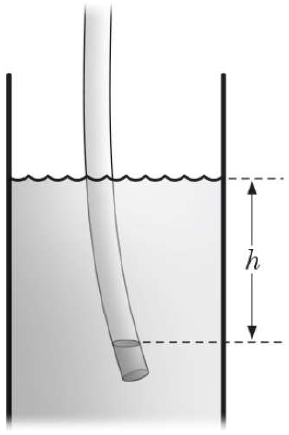
\includegraphics{fig/Nivel/Altura.PNG}
        \caption{Medición de Nivel}
        \label{fig:altura}
    \end{figure}
    \item Registre la presión P (KPa) y el nivel h (cm) como se indica en la tabla No. 1. Además registre la temperatura ambiente. 
    \begin{table}[!ht]
        \centering
        \begin{tabular}{c|c}
            \textbf{Nivel[cm]} & \textbf{Presión[kPa]} \\
            \hline
             0 & \\
             4 & \\
             8 & \\
             12 & \\
             16 & \\
             20 & \\
             24 & \\
             28 & \\
        \end{tabular}
        \caption{Presión vs nivel en una columna de agua}
        \label{tab:my_label}
    \end{table}
    \item Descienda el tubo dentro del agua cuatro centímetros adicionales.
    \item Repita el paso anterior hasta que haya registrado presiones para seis niveles: 0 cm, 4 cm, 8 cm, 12 cm, 16 cm y 20 cm.
    \item Guarde los datos en un archivo \emph{.csv} y genere el mismo gráfico visto en el software "Pasco Capstone" durante el experimento.
    \item Realice el siguiente análisis en las tres tomas de datos.
\end{enumerate}


\subsection{Análisis}
\begin{enumerate}
    \item Genere la curva de mejor ajuste realizada en el punto i del apartado de procedimiento. Determine y anote la ecuación de la línea.
    \item ¿El gráfico de presión versus nivel produce una relación lineal? Explique. 
    \item La presión estática está relacionada con el nivel mediante la ecuación:
    \begin{equation}
        P=P_0+\rho * h * g
    \end{equation}
    
    Donde $P$ es la presión, $P_0$ es la presión inicial, $rho$ es la densidad del fluido, $g$ es la aceleración de la gravedad y $h$ es el nivel/profundidad. A partir del gráfico lineal que relaciona la presión con el nivel, extrapole el valor para la densidad del valor del fluido en el depósito (agua). Muestre su cálculo.
    \item Si el valor teórico de la densidad de agua es 1,000 kg/m3, calcule el porcentaje de error entre el valor experimental y el valor actual
    \begin{equation}
        Porcentaje_{error}=\frac{|Actual-Experimental|}{Actual}\times 100
    \end{equation}
    \item Si se realiza el mismo experimento utilizando yodo líquido (densidad ≈ 4,900 kg/m3) en lugar de agua, ¿cómo sería diferente un gráfico de presión versus nivel?
\end{enumerate}

%	Mediciones de nivel
%----------------------------------------------------------------------------------------


% ------------------------------------------------------------
\chapter{Medición de aceleración}
\section{\obj}
\capacidad
\begin{itemize}
\item Medir la aceleración lineal de un cuerpo.
\item Determinar la velocidad y la posición a partir de los datos de aceleración
\end{itemize}

\section{\mat}
\begin{itemize}
\item 1 interfaz ScienceWorkshop\,\textregistered\,750
\item 1 sensor de aceleración, CI-6558
\item 1 nivel
\item 1 riel para carrito PASCO
\item 1 carrito ME-9454, con hilo de nylon
\item 3 masas de 50 gramos
\end{itemize}


\section{\pro}
\subsection{Experimento}
\begin{enumerate}
    
    \item Arme el riel y procure que quede a nivel, coloque el limite para el carrito a los 100cm
    \item Fije el sensor de aceleración al carrito
    \item Conecte el sensor a la interfaz
    \item Fije la masa al cable de nylon
    \item Configure la toma de datos a una frecuencia de 1kHz, condición de inicio: aumenta por encima de 0.1, condición de parada: cae por debajo de -1
    \item Presione el botón registrar y luego utilice la pesa pequeña para liberar el carrito
    \item Repita la toma 3 veces, una por cada masa
    \item Guarde los datos en un archivo \emph{.csv}
    \item Realice el siguiente análisis en las tres tomas de datos.
\end{enumerate}


\subsection{Análisis}
\begin{enumerate}
    \item Genere los gráficos de aceleración vrs. tiempo, velocidad vrs. tiempo y desplazamiento vrs. tiempo usando los datos de las tomas anteriores
    \item ¿Es el comportamiento esperado? Analice.
    \item Compare con el desplazamiento real realizado y discuta a que se debe la diferencia. 
    \item ¿Porque se produce oscilación en los valores del sensor al inicio de la toma de datos? Explique. 
\end{enumerate}

% ------------------------------------------------------------
\chapter{Medición de óptica}
\section{\obj}
\capacidad
\begin{itemize}
\item Comprender el funcionamiento de los sensores ópticos. 
\item Estudiar de forma experimental cómo la intensidad de luz cambia con la distancia.
\end{itemize}

\section{\mat}
\begin{itemize}
\item 1 interfaz ScienceWorkshop\,\textregistered\,750
\item 1 sensor de luz, CI-6504A
\item 1 nivel
\item 1 riel para carrito PASCO
\item 1 carrito, ME-9439
\item 1 diodo laser
\item Laminas de madera
\end{itemize}


\section{\pro}
\subsection{Montaje}
\begin{enumerate}
    
    \item Inserte el sensor de luz CI-6504A en uno de los canales analógicos de la Interfaz 750 de \textit{PASCO}
    \item Seleccione la Interfaz \textit{ScienceWorkshop} 750 en configuración del hardware en PASCO Capstone, asegúrese de que el dispositivo esté encendido
    \item Haga click en el canal analógico donde está conectado el sensor de luz CI-6504A. Seguidamente seleccione \textit{Sensor de luz}.
    \item Configure el riel de baja fricción. Coloque el carrito de baja fricción y encima del carrito, coloque una lámina de madera. Seguidamente, ubique el sensor de luz, CI-6504A. Coloque dos laminas adicionales en el riel de baja fricción, y ubique el Diodo Láser sobre dichas laminas. \textbf{Recomendación:} puede fijar el sensor utilizando doble cinta. 
    \item Cree una tabla y un gráfico en el software \textit{Pasco Capstone}, para observar en tiempo real la recolección de los datos, con Intensidad de Luz en el eje de las ordenadas y Distancia en el eje de las abscisas. En este punto del procedimiento, el sistema recolector de datos deberá estar configurado en el modo de muestreo manual, con la entrada manual de datos. Titule la entrada manual de datos como “Distancia” con unidades de metros (m).
    \item Muestre la intensidad de luz en una pantalla digital (display) del software \textit{Pasco Capstone}.
    \item Si el sensor cuenta con rangos diferentes de ajustes, comience con el rango medio, accionando la perilla con la que cuenta el sensor en uno de los costados.
    \item Encienda la fuente de luz. \textbf{Nota:} Al conectar el diodo láser se deberá tener mucho cuidado con no apuntar a la cara de de otros miembros.
    \item Deslice el sensor de luz, sobre el riel de baja fricción, hacia adelante y atrás, para determinar el punto donde los valores de intensidad de luz comiencen a cambiar. Esta, va a ser la distancia mínima en la que el sensor de luz debe estar alejado de la fuente de luz. Usted puede necesitar cambiar la sensibilidad del sensor de luz, si obtiene una distancia mayor a los 50 cm desde la fuente de luz. \textbf{Recomendación}: Comience probando con una distancia inicial de separación de 20 cm entre el sensor y la fuente de luz.
\end{enumerate}

\subsection{Toma de datos}
\begin{enumerate}
    \item Inicie la recolección manual de datos. 
    \item En el punto e del apartado de Montaje se especificó la elaboración de un gráfico de Intensidad de Luz versus Distancia, el cual se debería estar observando en tiempo real.
    \item Registre el primer punto de datos muestreados manualmente y luego digite la distancia correspondiente, en metros, entre el Diodo laser y el elemento sensor en el sensor de luz. \textbf{Nota:} El elemento sensor de luz en el sensor de luz está justo detrás del extremo inferior del tubo negro en la parte frontal del sensor.
    \item Aleje el sensor de luz 2.0 cm de la fuente de luz y luego registre otro dato manualmente. Digite la distancia correspondiente, en metros, entre el Diodo laser y el elemento sensor en el sensor de luz.
    \item Repita el paso anterior hasta que se hayan recolectado al menos 10 datos distintos.
\end{enumerate}

\subsection{Análisis}
\begin{enumerate}
    \item Describa el gráfico obtenido durante la recolección de datos. Sea sintético en su descripción. Incluya observaciones tales como: ¿La intensidad aumentó o disminuyo conforme se alejaba el sensor de la fuente de luz, y el gráfico fue lineal o curvo? Si fue curvo, ¿cuál es la relación matemática que produce la forma del gráfico?
    \item Investigue sobre la Ley del cuadrado inverso. Deduzca la expresión matemática que ejemplifica la ley (la intensidad de la luz es inversamente proporcional al cuadrado de la distancia de la fuente de luz).
    \item Copie los datos obtenidos en la tabla efectuada anteriormente en un procesador matemático y cree dos nuevos sets de datos, para los inversos de la distancia: $\frac{1}{[Distancia(m)]}$ y $\frac{1}{[Distancia(m)]^2}$.
    \item De los datos generados anteriormente, realice los siguientes dos gráficos: uno con Intensidad de Luz en el eje de las ordenas y el inverso de la distancia, $\frac{1}{[Distancia(m)]}$, en el eje de las abscisas. Adicionalmente, con Intensidad de Luz en el eje de las ordenas y el inverso de la distancia al cuadrado, $\frac{1}{[Distancia(m)]^2}$, en el eje de las abscisas.
    \item ¿Alguno de los gráficos produce una línea recta? ¿Cuál es el significado de su respuesta?
\end{enumerate}

\renewcommand{\appendixname}{Taller}
\renewcommand{\appendixtocname}{Taller}
\renewcommand{\appendixpagename}{Taller}

\appendix
\renewcommand{\thechapter}{\Roman{chapter}}

%	Taller de sensores analógicos
%----------------------------------------------------------------------------------------


% ------------------------------------------------------------
\chapter{Sensores digitales}
\section{\obj}
\capacidad
\begin{itemize}
\item Adquirir datos de distancia usando un sensor de tiempo de viaje (ToF) conectado a una tarjeta de desarrollo Arduino Mega 2560.
\item Definir el tiempo entre mediciones usando una interrupción de \SI{0.1}{\second}.
\item Leer los datos de distancia enviados por medio de comunicación serial usando Python y graficar en tiempo real.
\item Utilizar una declaración \emph{match-case} en Python para realizar la decodificación de los valores de distancia
\end{itemize}

\section{Introducción}

Un sensor de distancia de tiempo de vuelo (time-of-flight) es un dispositivo utilizado para estimar la distancia a un cuerpo calculando el tiempo de vuelo de un haz de luz generada por un laser, esto es, el tiempo transcurrido entre la emisión y la recepción del haz. Para esta experiencia se utilizará un sensor VL53LOX. 

La conexión con el Arduino MEGA 2560 se muestra en la Figura \ref{fig:e2f1}, el sensor envia los datos usando el protocolo de comunicación I2C    


\section{\mat}
\begin{itemize}
\item 1 Arduino Mega 2560.
\item 1 breadboard.
\item 1 sensor de distancia VL53LOX.
\item Cables de conexión macho-macho.
\end{itemize}

\section{\pro}
\begin{enumerate}
\item Realice las conexiones del circuito tal y como se indica en la Figura \ref{fig:e2f1}.

\begin{figure}[H]
    \tikzset{comm/.style={muxdemux, muxdemux def={Lh=5, Rh=5, NL=2, NB=0, NR=0, w=2}}}
    \tikzset{VL53LOX/.style={muxdemux, muxdemux def={Lh=5, Rh=5, NL=0, NB=0, NR=6, w=2}}}
    \centering
    \begin{circuitikz} 
        \draw (0,0) node[comm] (m){\rotatebox{90}{\small communication}}
        ;
        \draw (m.blpin 1) node[above left]{\small SDA (20)};
        \draw (m.blpin 2) node[above left]{\small SCL (21)};
        \draw (-5,-3) node[VL53LOX,rotate=90] (s){\rotatebox{-90}{\small VL53LOX}}
        (s.brpin 1) node[above right,rotate=90]{\scriptsize Vin}
        (s.brpin 2) node[above right,rotate=90]{\scriptsize GND}
        (s.brpin 3) node[above right,rotate=90]{\scriptsize SCL}
        (s.brpin 4) node[above right,rotate=90]{\scriptsize SDA}
        (s.brpin 5) node[above right,rotate=90]{\scriptsize GPIO1}
        (s.brpin 6) node[above right,rotate=90]{\scriptsize XSHUT}
        ;
        \draw
        (0,2.5) node[ground]{}
            to[V] 
        (0,4.5) node[above,xshift=-11mm]{5V} 
            --
        (-0.8,4.5)
        (0,2.5) node[above,xshift=-11mm]{GND} 
            --
        (-0.8,2.5)
        ;
        \draw[blue]
        (-0.8,4.5)
            -|
        (s.brpin 1)
        ;
        \draw[green]
        (-0.8,2.5)
            -|
        (s.brpin 2)
        ;
        \draw[red]
        (m.blpin 1) --++ (-2,0) -| (s.brpin 4)
        ;
        \draw[brown]
        (m.blpin 2) --++ (-2,0) -| (s.brpin 3)
        ;
        \draw[dashed,blue]
        (-2.5,6) -- (1,6)node[midway, below]{MEGA 2560} -- (1,-1.5) -- (-2.5,-1.5) -- cycle;
    \end{circuitikz}
    \caption{Conexión de módulo de lectura de termopar basado en MAX31855.}
    \label{fig:e2f1}
\end{figure}

\item Instale la librería \emph{Adafruit\_VL53L0X} usando el administrador de librerias de Arduino IDE. 
\item Instale la librería \emph{TimerInterrupt.h} usando el administrador de librerias de Arduino IDE.



\item Copie el siguiente código en el IDE de Arduino (el codigo se puede encontrar en: \href{https://github.com/DeltaLabo/talleres}{talleres})
\begin{lstlisting}[language=Arduino,numbers=none, showstringspaces=false]
// Incluir librería para el sensor
#include "Adafruit_VL53L0X.h"
// Hacer un #define para que la libreria TimerInterrupt cargue el Timer3
#define USE_TIMER_3     true
// Incluir librería para interrupciones basadas en tiempo
#include "TimerInterrupt.h"

// Definir variable para guardar la medición del sensor
int distance = 0;
// Definir variable para levantar la bandera del timer
bool timer_flag = true;
// Definir el encabezado y la cola del la trama que se enviará por serial
uint8_t header[2]={0xAA,0xDD};
uint8_t footer[2]={0xAA,0xFF};  

// Definir el intervalo del timer en milisegundos
#define TIMER_INTERVAL_MS        100

// Definir una instacia del sensor del tipo "Adafruit_VL530X" y con el nombre "sensor"
Adafruit_VL53L0X sensor = Adafruit_VL53L0X();

void setup() {
  // Inicializar el puerto serial
  Serial.begin(9600);
  // Inicializar el sensor
  if (!sensor.begin()) {
    Serial.println("No se ha podido iniciar el sensor.");
    while(1);
  }
  // Iniciar medición continua
  sensor.startRangeContinuous();
  // Inicializar el Timer 3
  ITimer3.init();
  // Asignar una interrupción por tiempo que ejecuta la función "TimerHandler"
  if (ITimer3.attachInterruptInterval(TIMER_INTERVAL_MS, TimerHandler))
  {
    Serial.print(F("Starting  ITimer3 OK, millis() = ")); Serial.println(millis());
  }
  else
    Serial.println(F("Can't set ITimer3. Select another freq. or timer"));
}

void TimerHandler()
{
  // Cuando se activa la función se sube la bandera
  timer_flag = true;
}

void loop() {
  if (timer_flag)
  {
    // Se realiza medición y se convierte a centimetros
    distance = sensor.readRange()/10;
    // Se establece como máximo 150 cm en caso que se alcance
    if (distance >= 150) distance = 150;
    // Se construye una trama con los datos:
    // OxAA 0xDD (4 bytes con el dato medido, MSBF) OxAA 0xFF
    Serial.write(header,2);
    Serial.write( (distance>>8) & 0xFF);
    Serial.write( (distance) & 0xFF);
    Serial.write(footer,2);
    // Se baja la bandera del timer
    timer_flag = 0;
  }
}
\end{lstlisting}
\item Analice cada linea de código y cuando entienda su funcionamiento corra el \emph{sketch} usando el botón \emph{Upload}
\item Haga contacto con el encapsulado del sensor de forma que su dedos calienten el sensor, observe como cambia el valor en la terminal. 
\item Instale las librerías \emph{pyserial}, \emph{matplotlib}, \emph{drawnow} y \emph{datetime} en Python para ser utilizadas luego.
\item Copie el siguiente código en su IDE de Python.

\begin{lstlisting}[language=Python, numbers=none, showstringspaces=false]
import serial
import matplotlib.pyplot as plt
from drawnow import drawnow
from datetime import datetime

ser = serial.Serial('COM11', baudrate=9600,
bytesize=8, parity='N', stopbits=1, timeout=1.5)
ser.close()
ser.open()
ser.flush()
distance = 0
past_time = datetime.now()
seconds = 0

time_data = []
dist_data = []

plt.ion()
fig = plt.figure()

def dist_figure():
    ax1 = plt.subplot()
    plt.plot(time_data[-100:],dist_data[-100:])
    ax1.set(xlabel='time (s)', ylabel='distance (cm)',
       title='VL53LOX measurements')


while(True):
    recep = ser.read(1)
    match recep:
        case b'\xAA':
            if ser.read(1) == b'\xDD':
                distance = int.from_bytes(ser.read(2), 'big')
                tiempo_actual = datetime.now()
                deltat = (tiempo_actual - past_time).total_seconds()
                past_time = tiempo_actual
                seconds += deltat
                time_data.append(seconds)
                dist_data.append(distance)
                drawnow(dist_figure)

\end{lstlisting}
\item Asegurese de utilizar el mismo puerto común tanto en Arduino como en Python. En caso de ser distintos, modifique en la línea 6 del código de Phyton.

\end{enumerate}
\end{document}